\documentclass{standalone}

\usepackage{pgfplots}


\begin{document}
%  \pgfplotsset{grid style={dashed,gray}}
  \pgfplotsset{major grid style={dashed,red}}
  \pgfplotsset{minor grid style={dotted,gray}}
  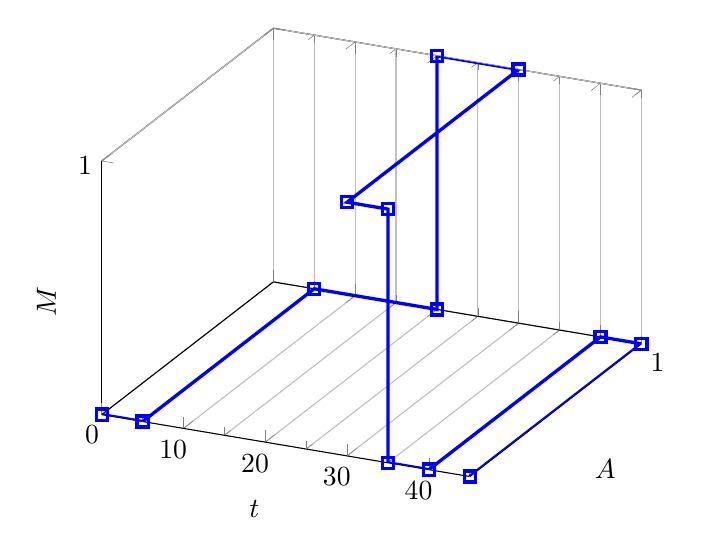
\begin{tikzpicture}
%    \pgfdeclareplotmark{ball}{%
%      \shade[draw=none,shading=ball] (0,0) circle (\pgfplotmarksize);
%    }

    \begin{axis}[grid=both,
      xtick={0,10,...,40},
      minor xtick={5,15,...,45},
      ytick={1},
      ztick={1},
      xlabel=$t$,
      ylabel=$A$,
      zlabel=$M$,
      scale=1,
      enlargelimits=0
      ]
      \addplot3[very thick, blue, mark=square] coordinates {(0,0,0)
        (5,0,0) (5,1,0)
        (20,1,0) (20,1,1)
        (30,1,1) (30,0,1)
        (35,0,1) (35,0,0)
        (40,0,0) (40,1,0)
        (45,1,0) (45,0,0)
      };
    \end{axis}
  \end{tikzpicture}
\end{document}

\begin{comment}
\usepackage{tikz}   %TikZ is required for this to work.  Make sure this exists before the next line
\usetikzlibrary{plotmarks}

\usepackage{tikz-3dplot} %requires 3dplot.sty to be in same directory, or in your LaTeX installation
\usepackage{pgfplots}

\usepackage[active,tightpage]{preview}  %generates a tightly fitting border around the work
\PreviewEnvironment{tikzpicture}
\setlength\PreviewBorder{2mm}

\begin{document}
%Angle Definitions
%-----------------

%set the plot display orientation
%synatax: \tdplotsetdisplay{\theta_d}{\phi_d}
\tdplotsetmaincoords{60}{60}

%define polar coordinates for some vector
%TODO: look into using 3d spherical coordinate system
\pgfmathsetmacro{\rvec}{.8}
\pgfmathsetmacro{\thetavec}{30}
\pgfmathsetmacro{\phivec}{60}

%start tikz picture, and use the tdplot_main_coords style to implement the display 
%coordinate transformation provided by 3dplot
\begin{tikzpicture}[tdplot_main_coords]

%set up some coordinates 
%-----------------------
\coordinate (O) at (0,0,0);

%determine a coordinate (P) using (r,\theta,\phi) coordinates.  This command
%also determines (Pxy), (Pxz), and (Pyz): the xy-, xz-, and yz-projections
%of the point (P).
%syntax: \tdplotsetcoord{Coordinate name without parentheses}{r}{\theta}{\phi}
\tdplotsetcoord{P}{\rvec}{\thetavec}{\phivec}

%draw figure contents
%--------------------

%draw the main coordinate system axes
\draw[thick,->] (0,0,0) -- (10,0,0) node[anchor=north east]{$t$};
\draw[thick,->] (0,0,0) -- (0,1,0) node[anchor=south west]{$A$};
\draw[thick,->] (0,0,0) -- (0,0,1) node[anchor=south]{$M$};

%\draw[mark=square*, mark options={fill=white}] (0,0,0) -- (1,0,0) -- (1,1,0) -- (2,1,0) -- (2,1,1);
%\addplot3 coordinates {(0,0,0) -- (1,0,0) -- (1,1,0) -- (2,1,0) -- (2,1,1)};

%draw a vector from origin to point (P) 
\draw[-stealth,color=red] (O) -- (P);

%draw projection on xy plane, and a connecting line
\draw[dashed, color=red] (O) -- (Pxy);
\draw[dashed, color=red] (P) -- (Pxy);

%draw the angle \phi, and label it
%syntax: \tdplotdrawarc[coordinate frame, draw options]{center point}{r}{angle}{label options}{label}
\tdplotdrawarc{(O)}{0.2}{0}{\phivec}{anchor=north}{$\phi$}


%set the rotated coordinate system so the x'-y' plane lies within the
%"theta plane" of the main coordinate system
%syntax: \tdplotsetthetaplanecoords{\phi}
\tdplotsetthetaplanecoords{\phivec}

%draw theta arc and label, using rotated coordinate system
\tdplotdrawarc[tdplot_rotated_coords]{(0,0,0)}{0.5}{0}{\thetavec}{anchor=south west}{$\theta$}

%draw some dashed arcs, demonstrating direct arc drawing
\draw[dashed,tdplot_rotated_coords] (\rvec,0,0) arc (0:90:\rvec);
\draw[dashed] (\rvec,0,0) arc (0:90:\rvec);

%set the rotated coordinate definition within display using a translation
%coordinate and Euler angles in the "z(\alpha)y(\beta)z(\gamma)" euler rotation convention
%syntax: \tdplotsetrotatedcoords{\alpha}{\beta}{\gamma}
\tdplotsetrotatedcoords{\phivec}{\thetavec}{0}

%translate the rotated coordinate system
%syntax: \tdplotsetrotatedcoordsorigin{point}
\tdplotsetrotatedcoordsorigin{(P)}

%use the tdplot_rotated_coords style to work in the rotated, translated coordinate frame
\draw[thick,tdplot_rotated_coords,->] (0,0,0) -- (.5,0,0) node[anchor=north west]{$x'$};
\draw[thick,tdplot_rotated_coords,->] (0,0,0) -- (0,.5,0) node[anchor=west]{$y'$};
\draw[thick,tdplot_rotated_coords,->] (0,0,0) -- (0,0,.5) node[anchor=south]{$z'$};

%WARNING:  coordinates defined by the \coordinate command (eg. (O), (P), etc.)
%cannot be used in rotated coordinate frames.  Use only literal coordinates.  

%draw some vector, and its projection, in the rotated coordinate frame
\draw[-stealth,color=blue,tdplot_rotated_coords] (0,0,0) -- (.2,.2,.2);
\draw[dashed,color=blue,tdplot_rotated_coords] (0,0,0) -- (.2,.2,0);
\draw[dashed,color=blue,tdplot_rotated_coords] (.2,.2,0) -- (.2,.2,.2);

%show its phi arc and label
\tdplotdrawarc[tdplot_rotated_coords,color=blue]{(0,0,0)}{0.2}{0}{45}{anchor=north west,color=black}{$\phi'$}

%change the rotated coordinate frame so that it lies in its theta plane.
%Note that this overwrites the original rotated coordinate frame
%syntax: \tdplotsetrotatedthetaplanecoords{\phi'}
\tdplotsetrotatedthetaplanecoords{45}

%draw theta arc and label
\tdplotdrawarc[tdplot_rotated_coords,color=blue]{(0,0,0)}{0.2}{0}{55}{anchor=south west,color=black}{$\theta'$}

\end{tikzpicture}

\end{document}
\end{comment}
